\chapter{Módulo servidor}
Para este proyecto se ha decidido crear un servidor propio con IP local. Es cierto que este servidor podría haberse alojado en algún hosting. Pero para asegurar la privacidad de los datos que publica el usuario de este monitor se ha decidido que lo mejor es alojar el servidor en una Raspberry Pi con IP local.

\section{Requisitos}
\subsection{Requisitos funcionales}

\begin{itemize}
	\item\textbf{RF1: } Ha de permitir al usuario consultar los consumos en un intervalo de fechas.
	\item\textbf{RF2: } Mostrar mediante una tabla los consumos ordenados por fecha y hora.
	\item\textbf{RF3: } En caso de mostrar una tabla muy extensa dividirla por páginas mediante un paginador.
	\item\textbf{RF4: } Mostrar la media de consumo durante las fechas especificadas por el usuario.
	\item\textbf{RF5: } Mostrar mediante un gráfico consumos del mes anterior y posterior al consultado por el usuario.
\end{itemize}

\subsection{Requisitos no funcionales}

\begin{itemize}
	\item\textbf{RNF1: } Hacer que el diseño de la web sea responsivo, es decir que se adapte a tamaños de pantalla diferentes para ajustarse a dispositivos móviles como smartphones o tablets o a ordenadores.
	\item\textbf{RNF2: } Persistencia de datos mediante una base de datos NoSql.
	\item\textbf{RNF3: } Se utilizarán tecnologías open source.
	\item\textbf{RNF4: } Garantizar la privacidad de los datos del usuario.
	\item\textbf{RNF4: } Compatibilidad con los navegadores.
\end{itemize}

\section{Backend}
La parte del Backend de la aplicación web está realizada con Flask \cite{Flask}. Se trata de un microframework para python que utiliza plantillas Jinja2 \cite{jinja2info}. Para una aplicación web pequeña como es el caso de la que se va a realizar para este proyecto nos ha parecido más apropiado utilizar este microframework ya que al contrario que otros framework como puede ser Django cuenta con con pocas características las cuales se pueden ir añadiendo mediante módulos los cuales en función de nuestras necesidades podremos ir añadiendo, sin embargo en un framework como Django \cite{Django} ya se incluyen todos estos componentes.

El motivo principal para escoger Flask frente a Django principalmente ha sido por el conocimiento previo que tenia adquirido en la asignatura desarrollo de aplicaciones para internet. También se había trabajado con Django en la asignatura infraestructura virtual pero en menor medida.

Para la persistencia de datos hemos utilizado bases de datos NoSQL más concretamente MongoDB, se trata de una base de datos orientada a documentos los datos se guardan en documentos BSON (una representación binaria de JSON) en lugar de en registros como ocurre en bases de datos convencionales. Esto permite introducir cualquier dato aunque se cambie el formato al contrario que en las bases de datos relacionales que es necesario seguir un esquema \cite{MongoDB}.

\section{Frontend}
Para realizar el frontend de la aplicación se han utilizado plantillas HTML 5 bootstrap para conseguir que el diseño de la web sea responsive. Al utilizar bootstrap conseguimos que el diseño de la web sea compatible con la mayoría de navegadores web \cite{Bootstrap}.
Se necesita además una herramienta open source para realizar las gráficas de consumo. Para ello se ha utilizado la herramienta Higcharts la cuál nos permite realizar gráficas utilizando JavaScript.

\section{Servidor}
Para alojar la aplicación web diseña para este proyecto no es necesario un servidor con demasiada potencia por lo tanto con alojar la web en una Raspberry Pi nos será más que suficiente.

\subsection{Sistema Operativo}

Como vamos a utilizar la Raspberry como servidor instalaremos un sistema operativo sin interfaz gráfica en concreto Raspbian Jessie Lite. Para instalar el sistema operativo en la tarjeta micro SD que introduciremos en la Raspberry tan solo tendremos que flashear la imagen que nos descargaremos de la web oficial de raspberry \cite{raspbianoficial}. Para flashear la imagen en la SD existen múltiples programas pero en mi caso he elegido utilizar Win32 disk imager \cite{Win32} un sencillo software open source disponible para múltiples plataformas que nos permitirá flashear la imagen en la tarjeta micro SD muy fácilmente. Hemos de tener en cuenta que previamente la tarjeta micro SD tendrá que estar formateada para lo cuál nos servirá cualquier software open source de los que están disponibles.

\subsection{Aprovisionamiento }
Para facilitar que cualquier persona interesada en el proyecto pueda montar de la forma más sencilla posible el servidor tan solo tendrá que descargarse mi repositorio de GitHub \url{https://github.com/Miguelmoral/ESP8266-energy-monitor}, los pasos a seguir para su descarga y puesta en funcionamiento son bastante sencillos \cite{repoESP}:

\begin{enumerate}
	\item\textbf{Instalar git: } Para poder descargar el repositorio de GitHub será necesaria la instalación de git en nuestra máquina con el comando:
	 \begin{listing}[style=consola, numbers=none]
	 	$ sudo apt-get update
		$ sudo apt-get install git
	\end{listing}
	\item\textbf{Descargar repositorio: } Una vez tenemos instalado git podremos descargar el repositorio introduciendo:
	
	\begin{listing}[style=consola, numbers=none]
	$ sudo git clone https://github.com/Miguelmoral/ESP8266-energy-monitor	
	\end{listing}
	
	\item\textbf{Instalar \textit{requirements}: } Una vez descargado este repositorio en el cuál se incluye todo lo necesario para el correcto funcionamiento del servidor el usuario tendrá que ejecutar el comando 
	
	\begin{listing}[style=consola, numbers=none]
		$ cd ESP8266-energy-monitor
		$ sudo make install
	\end{listing} 
		
\end{enumerate}

\subsection{Iniciar aplicación web }
El \textit{makefile} incluye además otro comando que permite directamente la ejecución de la aplicación web en el servidor, hay que tener en cuenta que para que este comando funcione previamente tendremos que haber realizado los pasos explicados anteriormente.

\begin{listing}[style=consola, numbers=none]
	$ make ejecutar
\end{listing} 

Al tratarse de una Raspberry Pi la cuál no dispone de pantalla sería interesante hacer que se ejecute automáticamente la aplicación web cada vez que arranquemos el sistema. Existen varias formas de conseguirlo \cite{rc.local}:

\begin{enumerate}
	\item Modificando el archivo rc.local.
	\item Modificando el archivo .bashrc.
	\item Añadir el \textit{script} o comandos que se quieran ejecutar al directorio /etc/init.d. 
	\item Utilizando los archivos systemd.
	\item Mediante el demonio cron. Tendremos que añadir los script que queramos ejecutar en el fichero crontab y especificar cuando queramos que se ejecuten. 
\end{enumerate}

 Para este proyecto se va a modificar el archivo rc.local de la máquina. Tan solo tendremos que abrir este archivo con un editor de textos con permisos root para poder editarlo e incluir antes de exit 0 el comando que queramos que ejecute la máquina cada vez que se encienda en nuestro caso.

Abriremos un editor de textos para modificar el archivo rc.local con

\begin{listing}[style=consola, numbers=none]
	$ sudo nano rc.local
\end{listing} 

Y añadiremos la orden 

\begin{listing}[style=consola, numbers=none]
$ sudo python /home/pi/ESP8266-energy-monitor/web/main.py &
\end{listing} 

Quedándose el archivo rc.local de esta forma \ref{fig:rc.local}

\begin{figure}[H]
	\centering
	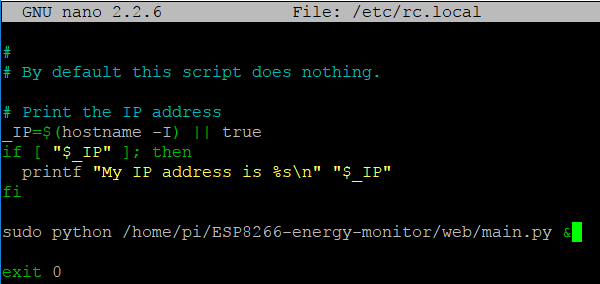
\includegraphics{imagenes/iniciaraplicacionweb2.png}
	\caption{rc.local Raspberry Pi}
	\label{fig:rc.local}
\end{figure}

\subsection{IP estática Raspberry }
Establecer una IP estática en la Raspberry no es totalmente necesario para el proyecto ya que podría funcionar perfectamente con una IP dinámica, pero por comodidad es preferible establecer una IP estática.

Para que el ESP8266 pueda mandar la información siempre a la misma IP y no tener que modificar el código del firmare cada vez que la Raspberry cambie de IP vamos a hacer que la IP de la Raspberry que por defecto es dinámica pase a ser estática de esta forma esta IP será siempre la misma la cuál le asignaremos nosotros modificando el archivo.

Tendremos que consultar algunos valores sobre nuestra conexión antes de modificar el archivo /etc/network/interfaces \cite{staticip}. Para ello utilizaremos el comando :
\begin{listing}[style=consola, numbers=none]
	$ netstat -nr 
\end{listing} 

Una vez sabemos cuál es nuestro broadcast range, subnet mask, gateway y destination podremos modificar el archivo /etc/network/interfaces de nuestra Raspberry para establecer una IP fija. Dependiendo de los valores que nos de dependiendo de la configuración de nuestra conexión tendremos que cambiar algunos datos a la hora de modificar este archivo pero en mi caso obtendríamos algo como lo que vemos en la imagen \ref{fig:confip}:

\begin{figure}[H]
	\centering
	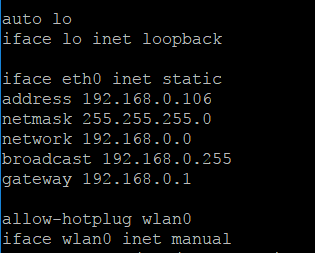
\includegraphics{imagenes/staticipconf.png}
	\caption{Configuración /etc/network/interfaces}
	\label{fig:confip}
\end{figure}


\subsection{Aspecto final de la página}

Tendremos una simple página de inicio donde podremos seleccionar de que fecha a que fecha queremos visualizar los datos:

\begin{figure}[H]
	\centering
	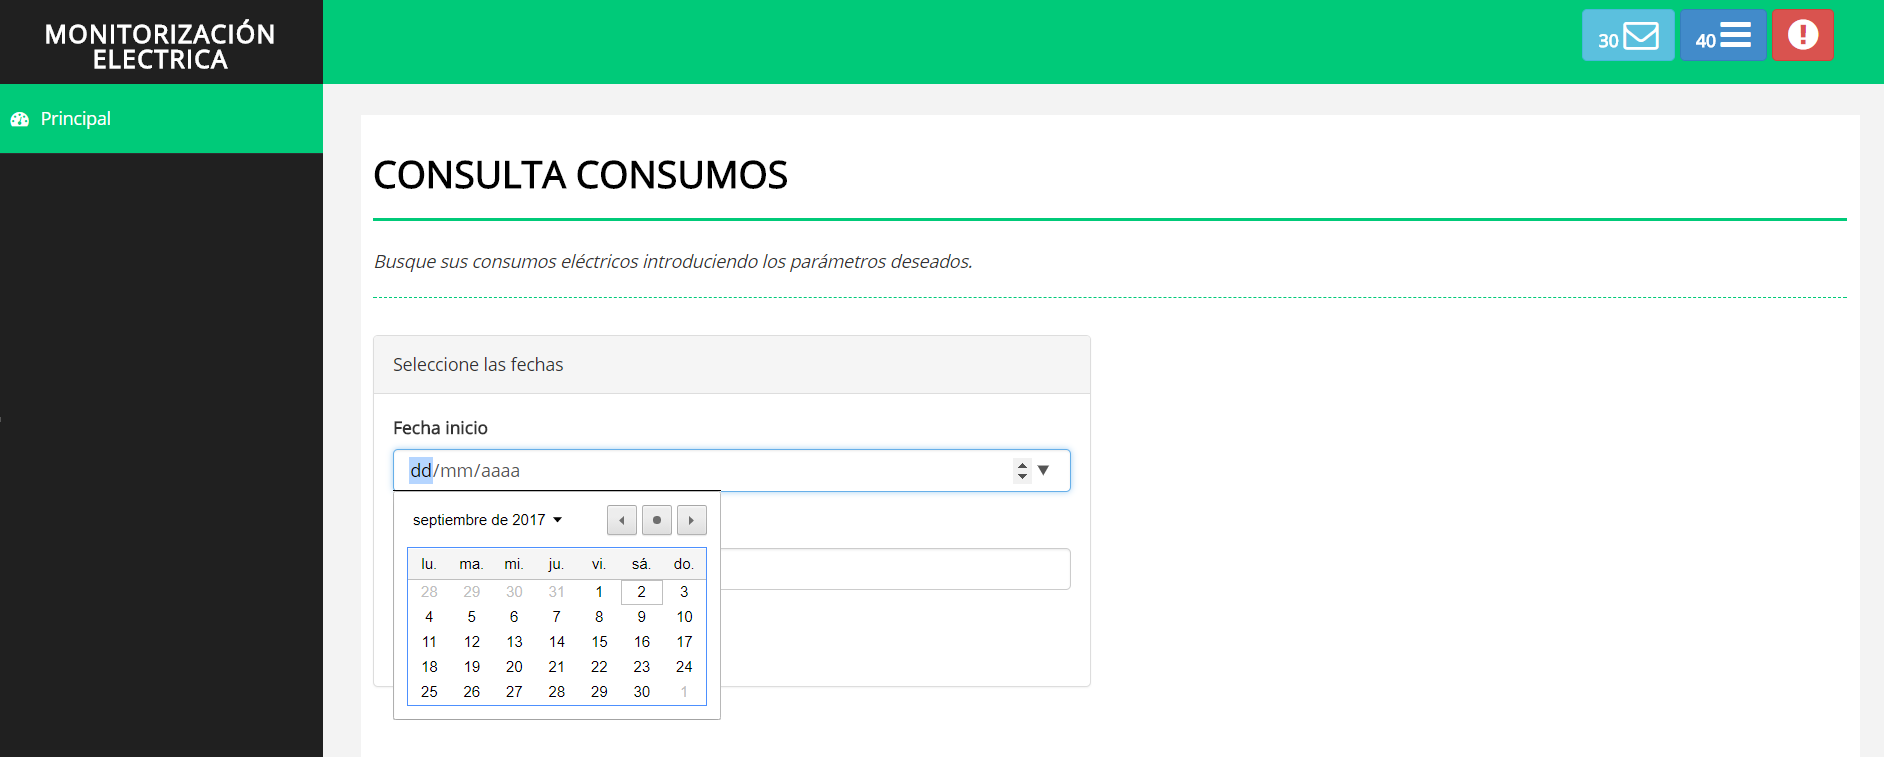
\includegraphics[scale=0.4]{imagenes/principalfecha.png}
	\caption{Página principal}
	\label{fig:principalweb}
\end{figure}

Al introducir las fechas veremos una tabla con los datos correspondientes a las fechas introducidas, un apartado que nos muestra la media tanto del irms como de la potencia consumida y una gráfica correspondiente a las medias de el mes anterior al consultado y el siguiente. En la gráfica mostrada tanto el mes siguiente como el anterior sale a 0 ya que durante esos meses no se recogieron muestras. En la gráfica (\ref{fig:tablaconsumos}) podemos ver los resultados de medir una bombilla de 60 W durante un periodo de tiempo. El paginador nos mostrará 10 entradas por página de esta forma se podrán visualizar los datos de una forma más clara que si se mostraran sin paginador. Además tendremos una gráfica que nos irá mostrando los últimos consumos que reciva el servidor (\ref{fig:grafultimos})

\begin{figure}[H]
	\centering
	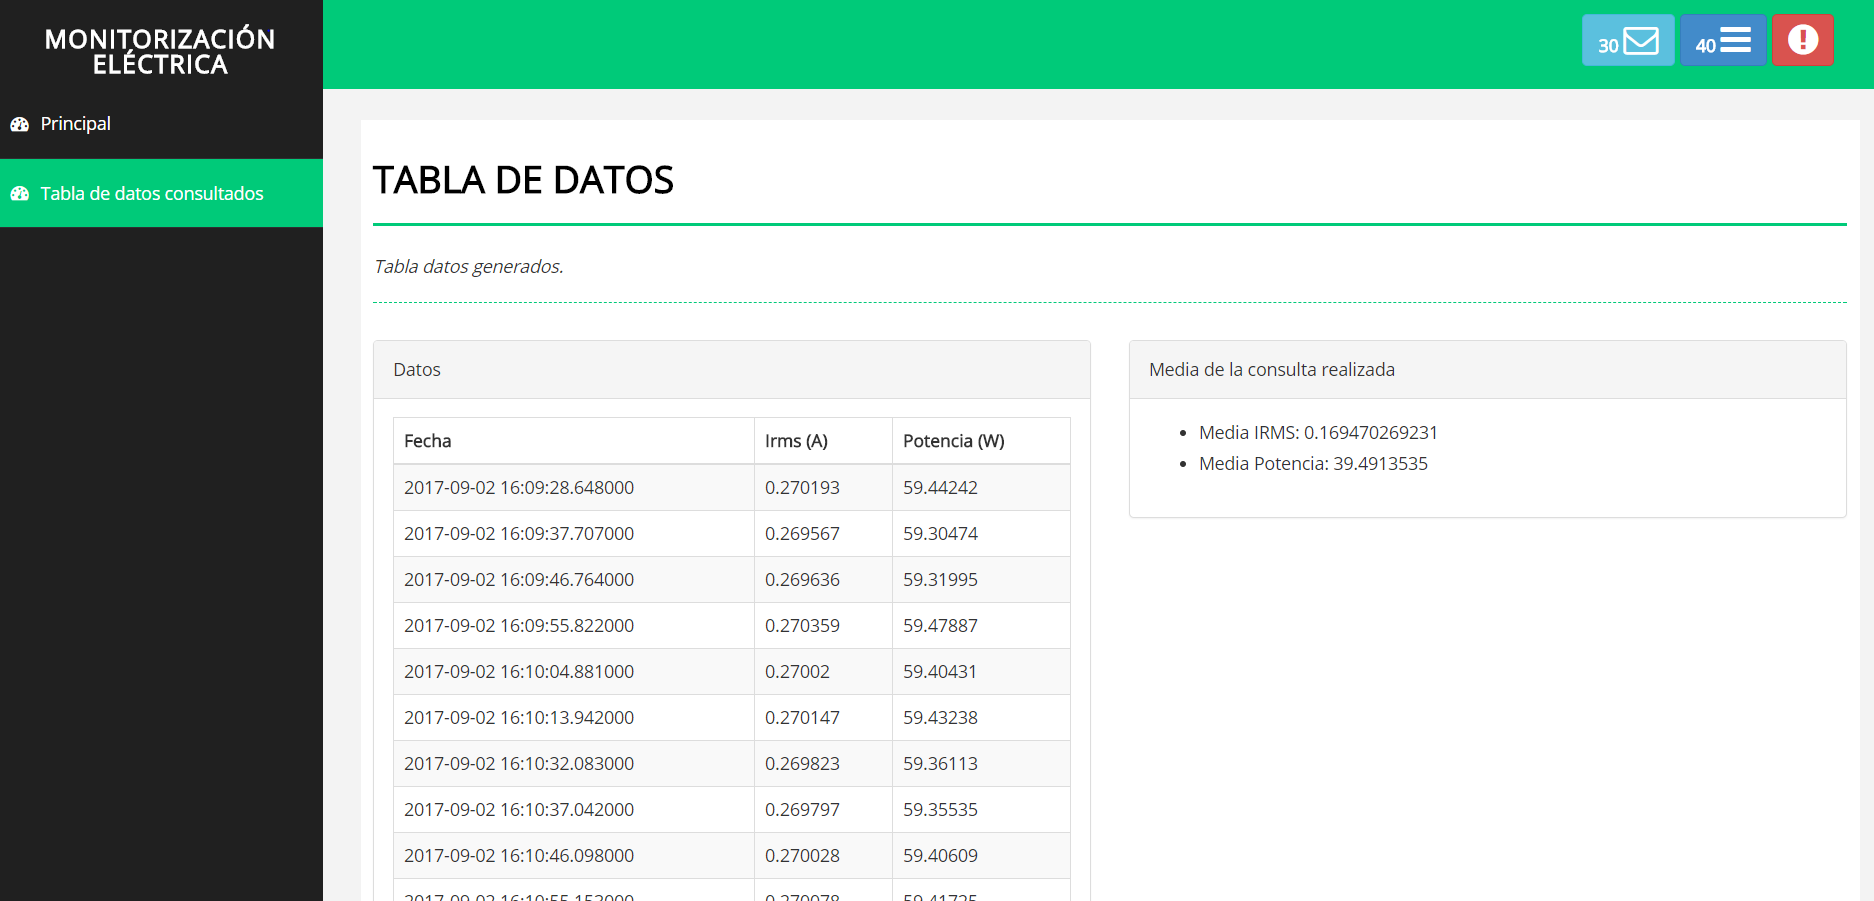
\includegraphics[scale=0.4]{imagenes/webbombillaconstante.png}
	\caption{Tabla de datos}
	\label{fig:tablaconsumos}
\end{figure}

\begin{figure}[H]
	\centering
	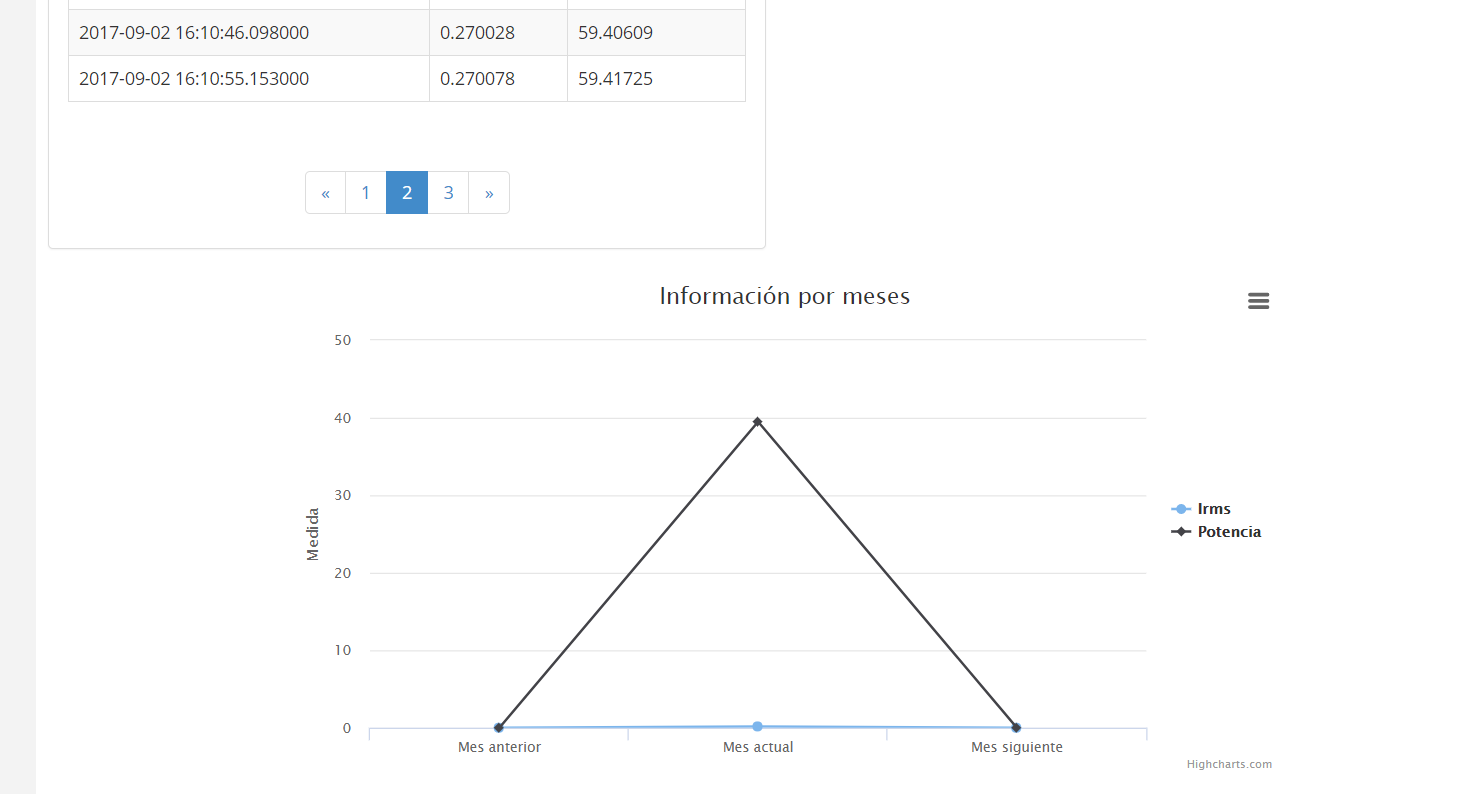
\includegraphics[scale=0.4]{imagenes/graficabombilla.png}
	\caption{Gráfica mensual}
	\label{fig:grafmensual}
\end{figure}

\begin{figure}[H]
\centering
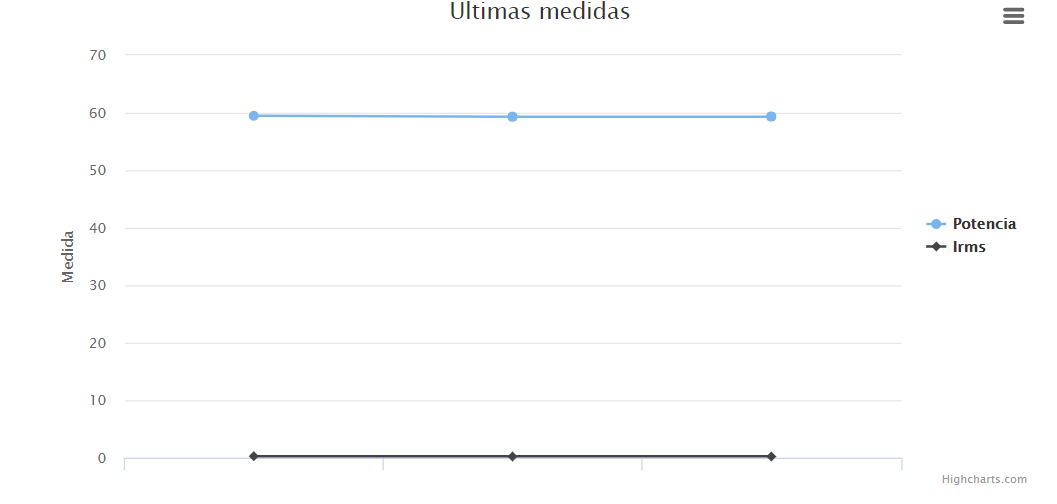
\includegraphics[scale=0.5]{imagenes/grafultima.png}
\caption{Gráfica ultimos consumos}
\label{fig:grafultimos}
\end{figure}

